\section{Theory}\label{sec:theory}

This section discusses the theory behind the models used in the 

\subsection{Regression model}

The regression model will be for the sake of convenience be expressed as the following expression
$$
\left(\vec{F}\circ \mathbf{A}\right)\vec{\beta}=\vec{y}+\vec{\varepsilon}
$$

Where $\vec{F}$ is a vector function with following domain $\vec{F}:\mathbb{R}^{m\times n}\to \mathbb{R}^{m\times p}$ where $m,p\in \mathbb{N}$, $\mathbf{A}$ is the data in matrix form with dimentions $\mathbb{R}^{m\times n}$, $\vec{\beta}$ is the regression terms, $\vec{y}$ is the target (TJM), and $\vec{\varepsilon}$ is the error from modelling. The $\circ$ operator is the composition of $\vec{F}$ and $\mathbf{A}$, is a short way of writing $\vec{F}(\mathbf{A})$.

\subsection{Rankin algorithmn}


\subsection{Long Short Term Memory model}

\begin{figure}[ht]
	\centering
	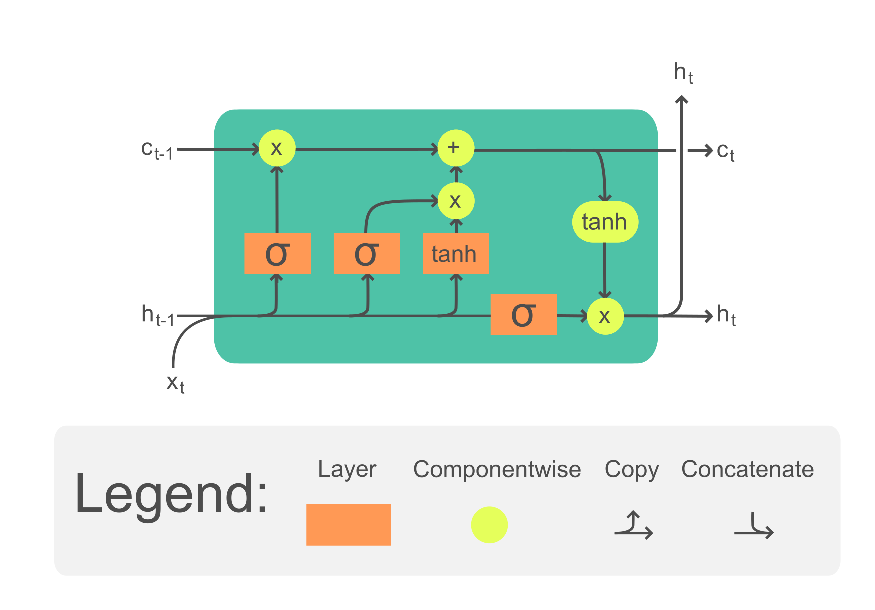
\includegraphics[width=0.7\linewidth]{figures/LSTM_Cell}
	\caption{LSTM cell  Artist: \textcite{chevalier_english_2018}}
	\label{fig:lstmcell}
\end{figure}

\subsection{ILSTM}

